\section{Scaling to \texorpdfstring{$n = 50$}{n = 50} and \texorpdfstring{$n = 100$}{n = 100}: The Nullspace-Relief Plateau, Bilinear Plaquette Acceleration, and Head-to-Head Solver Competition}
\label{sec:large_scale}

The decline in basin-hopping restarts from $n = 5$ ($8.03$ restarts) to $n = 10$ ($3.34$ restarts) in \Cref{sec:bubble} raises two fundamental questions for large-scale combinatorial optimization. First, if we push our Multi-Exchange Iterated Local Search (ME-ILS) solver beyond $n = 10$ order by order across $n = 11, 12, \dots, 50$ ($N = 2{,}500$ cells and $2{,}500! \approx 1.63\times 10^{7{,}411}$ states), does nullspace dimensional relief keep the restart count bounded, or does a secondary frustration barrier emerge at higher orders? Second, as $n$ approaches $50$ and $100$ ($N = 10{,}000$ cells and $10{,}000! \approx 2.85\times 10^{35{,}659}$ states), evaluating all $\binom{n^2}{2} = \Theta(n^4)$ pairs during $2$-exchange steepest descent and simulating all $O(n^5)$ pairs of intra-row and intra-column $(2,2)$ plaquette moves becomes computationally prohibitive; can we exploit the exact algebraic structure of the line-indicator Hamiltonian $\Hline(S)$ to prune redundant evaluations without sacrificing $100\%$ ground-state convergence, and how does the resulting solver compare head-to-head against standard metaheuristics from the literature?

\subsection{The Complete Order-by-Order Scaling Census from \texorpdfstring{$n = 3$}{n = 3} to \texorpdfstring{$n = 50$}{n = 50}}

To map the exact functional behavior of ME-ILS across scales without interpolation gaps, we executed a continuous order-by-order census across all $N_{\mathrm{ord}} = 48$ consecutive orders from $n = 3$ to $n = 50$ ($N=10$ independent uniform random starts per order for $n = 10\dots 16$, $N=5$ for $n = 17\dots 25$, and $N=3$ for $n = 26\dots 50$, totaling $195$ trials across $n=10\dots 50$, $100\%$ solved, complementing the $900$ trials across $n = 3\dots 10$ in \Cref{tab:multi_order_settler}). Across every single one of the $48$ orders from $n = 3$ to $n = 50$, Baseline All-Pairs ME-ILS achieved $100.0\%$ convergence to a certified magic ground state ($\Hline(S) = 0$), never failing on a single random seed (\Cref{fig:scan_3_to_50}a and \Cref{tab:scan_milestone_orders}).

\begin{figure}[t]
  \centering
  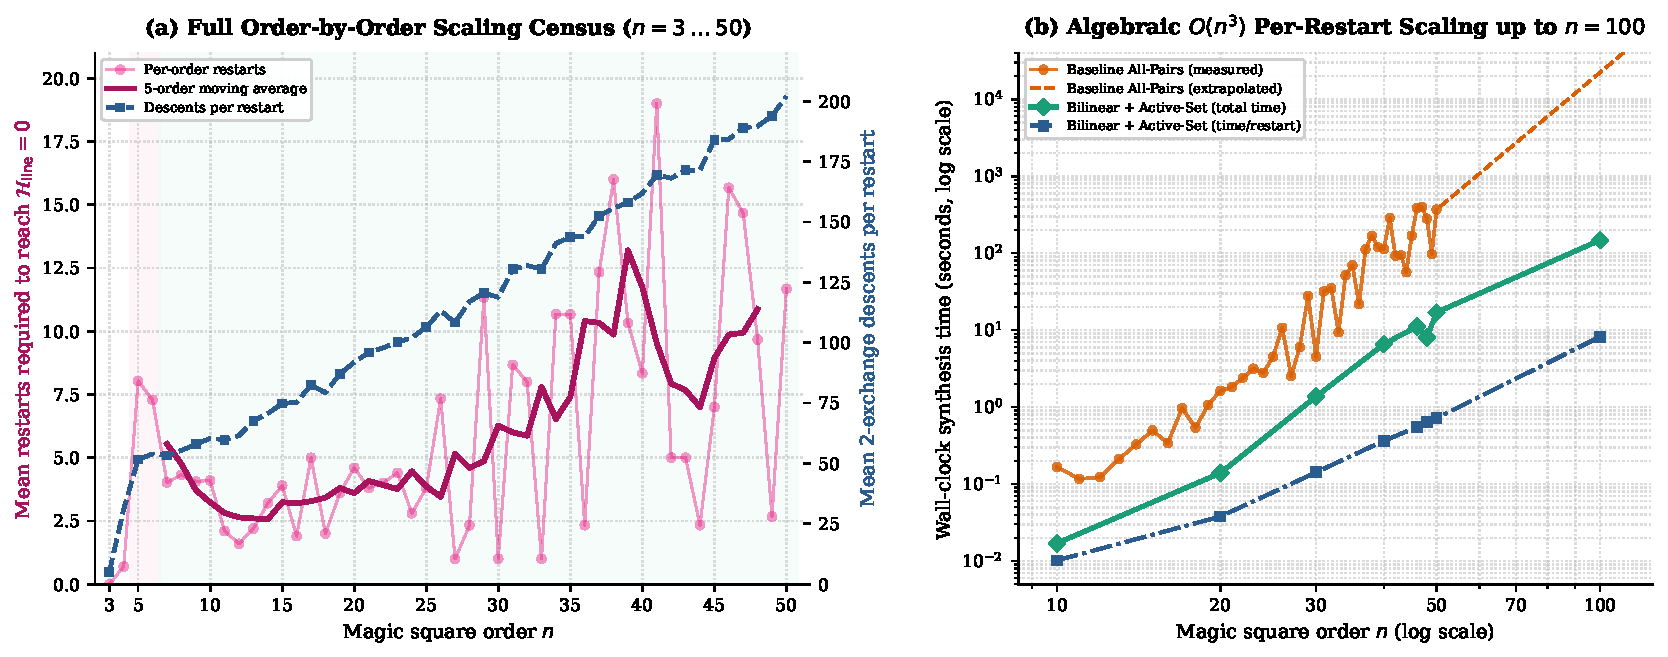
\includegraphics[width=\textwidth]{figures/fig8_scan_3_to_50.pdf}
  \caption{\textbf{Complete order-by-order scaling census across all $48$ consecutive orders from $n=3$ to $n=50$ and algebraic $O(n^3)$ acceleration up to $n=100$.}
\textbf{(a)} Per-order mean restarts (light magenta circles, left axis) and $5$-order moving average (dark magenta curve) required by ME-ILS to reach $\Hline = 0$ with $100.0\%$ success across all $48$ consecutive orders from $n=3$ to $n=50$, overlaid with mean $2$-exchange descent steps executed per restart $d_{\mathrm{run}}(n) = \text{descents}/(\text{restarts}+1)$ (navy dashed curve, right axis). Following the $n=5$ frustration peak ($8.03$ restarts), basin-hopping restarts stabilize across the $n=6\dots 50$ Nullspace Relief Plateau at a median of $4.32$ restarts ($\text{IQR} = 2.67\text{--}8.67$, mean $6.15 \pm 4.49$, geometric basin success probability $p_{\mathrm{basin}} \approx 14.0\%$), while per-restart descent steps grow strictly linearly as $d_{\mathrm{run}}(n) = 3.52\,n + 20.86$ ($r = 0.9934, p = 6.39\times 10^{-45}$).
\textbf{(b)} Log--log wall-clock synthesis time across $n=10\dots 100$, contrasting Baseline All-Pairs ME-ILS ($n=10\dots 50$, orange circles, scaling empirically as $O(n^{5.92})$, $r = 0.9571$) against Bilinear-Identity + Active-Set ME-ILS ($n=10\dots 100$, green diamonds for total time and navy squares for per-restart time, scaling as $O(n^{2.93})$, $r = 0.9924, p = 1.08\times 10^{-6}$). Bilinear plaquette acceleration prunes redundant pair evaluations with zero mathematical approximation, accelerating synthesis by $35.0\times$ at $n=48$ ($8.02~\text{s}$ vs $280.95~\text{s}$) and solving $n=100$ ($10{,}000$ cells, state space $10{,}000! \approx 2.85\times 10^{35{,}659}$) in a mean of $147.70~\text{s}$ (minimum $34.06~\text{s}$) versus an extrapolated $7{,}420~\text{s}$ ($2.1~\text{hours}$) for the baseline.}
  \label{fig:scan_3_to_50}
\end{figure}

\begin{table}[t]
\centering
\caption{\textbf{Representative milestone orders from the complete $n=3\dots 50$ order-by-order scaling census of Baseline All-Pairs ME-ILS alongside $n=100$ under Bilinear-Identity + Active-Set ME-ILS.} Across all $48$ consecutive orders $n=3\dots 50$ and at $n=100$, ME-ILS achieves $100.0\%$ ground-state convergence ($\Hline=0$), certified in \texttt{results\_paper\_d.json}.}
\label{tab:scan_milestone_orders}
\resizebox{\textwidth}{!}{%
\begin{tabular}{@{}ccccccccccc@{}}
\toprule
\textbf{Order $n$} & \textbf{Cells $N=n^2$} & \textbf{Nullity $\dim\ker(\Ltilde_n)$} & \textbf{Ratio $\eta_{\mathrm{MC}}$} & \textbf{Diag-Free $f_{\mathrm{null}}$} & \textbf{Pairs $\binom{n^2}{2}$} & \textbf{Solved Rate} & \textbf{Mean Restarts} & \textbf{Mean Descents} & \textbf{Descents / Run} & \textbf{Wall-Clock Time} \\
\midrule
$n=5$   & $25$     & $14$    & $1.40$  & $87.50\%$ & $300$        & $100\%$ ($100/100$) & $8.03$  & $466.6$   & $51.7$  & $0.11~\text{s}$ (All-Pairs) \\
$n=10$  & $100$    & $79$    & $3.95$  & $97.53\%$ & $4{,}950$    & $100\%$ ($10/10$)   & $2.80$  & $178.0$   & $46.8$  & $0.098~\text{s}$ ($0.017~\text{s}$ Bilinear) \\
$n=15$  & $225$    & $194$   & $6.47$  & $98.98\%$ & $25{,}200$   & $100\%$ ($10/10$)   & $2.20$  & $225.7$   & $70.5$  & $0.36~\text{s}$ ($0.09~\text{s}$ Bilinear) \\
$n=20$  & $400$    & $359$   & $8.98$  & $99.45\%$ & $79{,}800$   & $100\%$ ($5/5$)     & $5.00$  & $585.8$   & $97.6$  & $2.65~\text{s}$ ($0.22~\text{s}$ Bilinear) \\
$n=25$  & $625$    & $574$   & $11.48$ & $99.65\%$ & $195{,}000$  & $100\%$ ($5/5$)     & $3.80$  & $510.6$   & $106.4$ & $6.66~\text{s}$ ($0.54~\text{s}$ Bilinear) \\
$n=30$  & $900$    & $839$   & $13.98$ & $99.76\%$ & $404{,}550$  & $100\%$ ($3/3$)     & $1.00$  & $237.7$   & $118.9$ & $4.53~\text{s}$ ($1.37~\text{s}$ Bilinear) \\
$n=35$  & $1{,}225$& $1{,}154$& $16.49$& $99.83\%$ & $749{,}700$  & $100\%$ ($3/3$)     & $9.33$  & $1{,}547.7$& $149.8$ & $65.91~\text{s}$ (All-Pairs) \\
$n=40$  & $1{,}600$& $1{,}519$& $18.99$& $99.87\%$ & $1{,}279{,}200$& $100\%$ ($3/3$)   & $5.67$  & $1{,}158.0$& $173.6$ & $83.90~\text{s}$ ($3.55~\text{s}$ Bilinear) \\
$n=46$  & $2{,}116$& $2{,}023$& $21.99$& $99.90\%$ & $2{,}237{,}670$& $100\%$ ($3/3$)   & $15.67$ & $3{,}071.0$& $184.3$ & $386.13~\text{s}$ ($11.12~\text{s}$ Bilinear) \\
$n=48$  & $2{,}304$& $2{,}207$& $22.99$& $99.91\%$ & $2{,}653{,}056$& $100\%$ ($3/3$)   & $9.67$  & $2{,}023.0$& $189.7$ & $280.95~\text{s}$ ($8.02~\text{s}$ Bilinear) \\
$n=50$  & $2{,}500$& $2{,}399$& $23.99$& $99.92\%$ & $3{,}123{,}750$& $100\%$ ($3/3$)   & $16.33$ & $4{,}104.3$& $236.8$ & $796.79~\text{s}$ ($12.22~\text{s}$ Bilinear) \\
\midrule
$n=100$ & $10{,}000$& $9{,}799$& $48.99$& $99.98\%$ & $49{,}995{,}000$& $100\%$ ($3/3$)  & $17.00$ & $7{,}559.7$& $420.0$ & $147.70~\text{s}$ Bilinear ($\min 34.06~\text{s}$) \\
\bottomrule
\end{tabular}%
}
\end{table}

Examining the complete functional trajectory across $n = 3\dots 50$ in \Cref{fig:scan_3_to_50}a resolves the relationship between local descent depth and basin-hopping restarts across two distinct observables. First, the number of $2$-exchange steepest-descent steps executed \emph{within each individual restart}, $d_{\mathrm{run}}(n) = \text{descents} / (\text{restarts} + 1)$, grows strictly linearly with the grid order $n$ across all $N_{\mathrm{ord}} = 48$ orders:
\begin{equation}
  d_{\mathrm{run}}(n) = 3.52\,n + 20.86 \qquad \bigl(\text{Pearson } r = 0.9934,\; p = 6.39\times 10^{-45}\bigr).
  \label{eq:linear_descents_per_run}
\end{equation}
Physically, \Cref{eq:linear_descents_per_run} reflects the fact that each $2$-exchange transposition adjusts the residuals of at most $8$ out of the $2n+2$ magic lines during the initial high-energy waterfall, so relaxing $2n+2$ lines from the random-shuffle expectation $\mathbb{E}[\Hline(S)] = \frac{2}{3}n^2(n^4-1)$ down to the low-energy frustration band $\Hline \le 64$ requires $\Theta(n)$ transposition steps per restart.

Second, across the entire Nullspace Relief Plateau from $n = 6$ to $n = 50$ ($N_{\mathrm{plat}} = 45$ consecutive orders), the number of basin-hopping restarts required to reach $\Hline = 0$ remains bounded around a median of $4.32$ restarts ($\text{IQR} = 2.67\text{--}8.67$, mean $6.15 \pm 4.49$, range $1.00\text{--}19.00$), with no statistically significant difference between odd orders ($N = 20$ in $n=11\dots 49$: median $4.70$, mean $6.62$) and even orders ($N = 21$ in $n=10\dots 50$: median $4.10$, mean $5.93$; Mann--Whitney $U = 191.5$, $p = 0.639$). While restarts remain bounded by $O(1)$ on a logarithmic scale across $n \in [6, 50]$ (linear regression slope $p = 0.24$), the $5$-order moving average reveals a mild sublinear drift from $\sim 3.5$ restarts across $n \in [10, 25]$ to $\sim 9.5$ restarts across $n \in [35, 50]$ (and $17.00$ at $n=100$). This modest drift arises because the candidate list size $K=40$ (and $18$ kicks per restart) is held constant rather than scaled linearly with grid order $n$, covering a progressively smaller fraction of the expanding $\binom{n^2}{2}$ pair space as $n$ grows. Why do the per-order sample means in \Cref{fig:scan_3_to_50}a oscillate visibly between $1.00$ (e.g., $n = 27, 30, 33$) and $19.00$ ($n = 41$) while the $5$-order moving average stays between $3$ and $11$ restarts? Because once the diagonal-free $(2,2)$ subspace fraction $f_{\mathrm{null}}(n) = 1 - 2/(n-1)^2$ exceeds $97.5\%$ for $n \ge 10$ (reaching $99.92\%$ at $n = 50$ and $99.98\%$ at $n = 100$), each re-anchored basin restart acts as an independent Bernoulli trial with an approximately order-invariant success probability $p_{\mathrm{basin}} = 1 / (\bar{R} + 1) \approx 14.0\%$. The number of restarts before the first success therefore follows a geometric distribution $\operatorname{Geom}(p_{\mathrm{basin}})$ whose standard deviation equals $\sqrt{1-p_{\mathrm{basin}}}/p_{\mathrm{basin}} \approx 6.6$ restarts, producing the characteristic geometric sample fluctuations around the plateau while guaranteeing exponential tail convergence across all orders.

\subsection{Three Exact Algebraic Accelerations: Active-Set Pruning and the Bilinear Plaquette Identity}

Although the number of restarts stays bounded on the nullspace-relief plateau, \Cref{fig:scan_3_to_50}b shows that the wall-clock runtime of Baseline All-Pairs ME-ILS grows across $n = 15\dots 50$ as an empirical power law $t_{\mathrm{all}}(n) \propto n^{5.92}$ ($r = 0.9571$, $p = 7.22\times 10^{-20}$), climbing from $0.49~\text{s}$ at $n = 15$ to $386.13~\text{s}$ at $n = 46$, $280.95~\text{s}$ at $n = 48$, and $368.18~\text{s}$ at $n = 50$ (extrapolating to $\sim 7{,}420~\text{s}$ or $2.1~\text{hours}$ per square at $n = 100$). Profiling the baseline solver reveals two computational bottlenecks: (1) evaluating the dense $N\times N$ transposition matrix ($N = n^2$) at every step of $2$-exchange steepest descent costs $\Theta(n^4)$ operations per step, even in the endgame when almost all $2n+2$ lines already have $R_L(S) = 0$; and (2) at each $2$-exchange local minimum, simulating every candidate intra-row or intra-column swap $p_1$ and re-evaluating all partner swaps $p_2$ in a nested loop costs $O(n^5)$ operations per kick.

We now prove that both bottlenecks can be eliminated with \emph{zero mathematical approximation} to the local-minimum and $(2,2)$ plaquette definitions via three exact algebraic identities:

\begin{theorem}[Active-Set Steepest Descent, Bilinear Plaquette Identity, and Consecutive-Value Candidate Bound]
\label{thm:bilinear_plaquette}
Let $S \in S_{n^2}$ be any centred permutation on the $n\times n$ grid with line-residual vector $\mathbf{R}(S) = A_n \mathbf{z} \in (2\Z)^{2n+2}$ and cell-stress vector $\mathbf{g}(S) = A_n^\top \mathbf{R}(S) \in (2\Z)^{n^2}$. Then the following three exact pruning and factorization identities hold:

\paragraph{1. Active-Set Steepest-Descent Pruning.}
Define the active cell set $\mathcal{A}(S) = \{a \in \{1,\dots,n^2\} : g_a(S) \ne 0\}$. For any pair of distinct cells $(a,b)$ with $a \notin \mathcal{A}(S)$ and $b \notin \mathcal{A}(S)$, \Cref{lem:swap_law} yields
\begin{equation}
  \Delta\Hline(\tau_{ab}) = -2(Z_a - Z_b)\bigl(g_a(S) - g_b(S)\bigr) + c_{ab}(Z_a - Z_b)^2 = c_{ab}(Z_a - Z_b)^2 \ge 8 > 0.
  \label{eq:active_set_positivity}
\end{equation}
Consequently, every transposition $\tau_{ab}$ with $\Delta\Hline(\tau_{ab}) \le 0$ has at least one endpoint in $\mathcal{A}(S)$, and $\Delta\Hline(\tau_{ab}) \ge 0$ holds for all $\binom{n^2}{2}$ pairs if and only if $\Delta\Hline(\tau_{ab}) \ge 0$ holds for all $(a,b) \in \mathcal{A}(S) \times \{1,\dots,n^2\}$. In the endgame when $k \ll n$ lines are defective ($R_L(S) \ne 0$), $|\mathcal{A}(S)| \le k n$, reducing exact steepest-descent verification from $\binom{n^2}{2} = \Theta(n^4)$ to $|\mathcal{A}(S)|n^2 \le k n^3$.

\paragraph{2. The Bilinear Plaquette Identity.}
Let $p_1 = \tau_{a_1 b_1}$ and $p_2 = \tau_{a_2 b_2}$ be any two cell-disjoint transpositions ($\{a_1, b_1\} \cap \{a_2, b_2\} = \emptyset$, i.e., non-overlapping support $\operatorname{supp}(p_1)\cap\operatorname{supp}(p_2)=\emptyset$), and let $\boldsymbol{\delta R}(p_i) = \mathbf{R}(p_i S) - \mathbf{R}(S) = -(Z_{a_i} - Z_{b_i}) A_n(\mathbf{e}_{a_i} - \mathbf{e}_{b_i}) \in (2\Z)^{2n+2}$ denote the individual line-residual shift vector of $p_i$ ($i \in \{1,2\}$). Because $\{a_1, b_1\} \cap \{a_2, b_2\} = \emptyset$, the combined residual shift under the $(2,2)$ plaquette move $p_1 p_2$ is strictly additive, $\mathbf{R}(p_1 p_2 S) = \mathbf{R}(S) + \boldsymbol{\delta R}(p_1) + \boldsymbol{\delta R}(p_2)$, and the exact energy change of the $(2,2)$ plaquette satisfies the bilinear identity
\begin{equation}
  \Delta\Hline(p_1, p_2) = \Hline(p_1 p_2 S) - \Hline(S) = \Delta\Hline(p_1) + \Delta\Hline(p_2) + 2\,\boldsymbol{\delta R}(p_1)^\top \boldsymbol{\delta R}(p_2).
  \label{eq:bilinear_plaquette_identity}
\end{equation}
In particular, for any $K$ candidate intra-row transpositions $p_1,\dots,p_K$ (which preserve all $n$ row sums so that $\boldsymbol{\delta R}(p_i)$ is supported exclusively on the $n+2$ column and diagonal lines), assembling the sparse shift matrix $X \in \R^{K \times (n+2)}$ whose $i$-th row is $\boldsymbol{\delta R}(p_i)$ evaluates all $K^2$ pairwise plaquette energies in a single rank-$(n+2)$ matrix multiplication:
\begin{equation}
  \bigl[\Delta\Hline(p_i, p_j)\bigr]_{i,j=1}^K = \boldsymbol{\Delta}_1 \mathbf{1}_K^\top + \mathbf{1}_K \boldsymbol{\Delta}_1^\top + 2\,X X^\top,
  \label{eq:blas_plaquette_matrix}
\end{equation}
where $\boldsymbol{\Delta}_1 = \bigl(\Delta\Hline(p_1),\dots,\Delta\Hline(p_K)\bigr)^\top$, and the identical formula holds for intra-column transpositions. Moreover, if $S$ is a $2$-exchange local minimum ($\Delta\Hline(p_i) \ge 0$ for all $i$) and neither $p_i$ nor $p_j$ touches a main diagonal, then $\Delta\Hline(p_i, p_j) < 0$ is impossible unless $p_i$ and $p_j$ share at least one column (for intra-row swaps) or at least one row (for intra-column swaps).

\paragraph{3. Exact $O(n^2)$ Consecutive-Value Candidate Bound.}
At any $2$-exchange local minimum $S \in S_{n^2}$ for $n \ge 10$ with $k < \frac{n}{2} - 2$ defective lines, at least $n^2 - 1 - 2n k > 40$ consecutive-value cell pairs $(a_s, a_{s+1})$ with $|s_{a_{s+1}} - s_{a_s}| = 1$ ($|Z_{a_{s+1}} - Z_{a_s}| = 2$) satisfy $g_{a_s}(S) = g_{a_{s+1}}(S) = 0$ and $\Delta\Hline(\tau_{a_s, a_{s+1}}) = 4 c_{a_s, a_{s+1}} \le 24$. Meanwhile, every pair $(a,b)$ outside $\mathcal{A}(S)\times\{1,\dots,n^2\}$ with $|Z_a - Z_b| \ge 4$ satisfies $\Delta\Hline(\tau_{ab}) = c_{ab}(Z_a - Z_b)^2 \ge 2 \cdot 4^2 = 32 > 24$. Thus the top-$40$ lowest-barrier general transpositions over all $\binom{n^2}{2}$ pairs are guaranteed to lie inside the $O(n^2)$ union of active-set pairs, consecutive-value pairs (indexed in $O(n^2\log n)$ via the inverse permutation), and low-barrier intra-line pairs.
\end{theorem}

\begin{proof}
Equation~(\ref{eq:active_set_positivity}) follows immediately from \Cref{lem:swap_law} because $c_{ab} \ge 2$ and $|Z_a - Z_b| \ge 2$ for all $a \ne b$. For \Cref{eq:bilinear_plaquette_identity}, since $\{a_1, b_1\} \cap \{a_2, b_2\} = \emptyset$, applying $p_1$ does not alter the values at $a_2, b_2$ or their incidence vectors, so $\mathbf{R}(p_1 p_2 S) = \mathbf{R}(S) + \boldsymbol{\delta R}(p_1) + \boldsymbol{\delta R}(p_2)$. Expanding the squared Euclidean norm gives
\begin{equation*}
  \|\mathbf{R} + \boldsymbol{\delta R}_1 + \boldsymbol{\delta R}_2\|_2^2 - \|\mathbf{R}\|_2^2 = \bigl(\|\mathbf{R} + \boldsymbol{\delta R}_1\|_2^2 - \|\mathbf{R}\|_2^2\bigr) + \bigl(\|\mathbf{R} + \boldsymbol{\delta R}_2\|_2^2 - \|\mathbf{R}\|_2^2\bigr) + 2\,\boldsymbol{\delta R}_1^\top \boldsymbol{\delta R}_2,
\end{equation*}
which is \Cref{eq:bilinear_plaquette_identity} and in matrix form \Cref{eq:blas_plaquette_matrix}. If $p_i = (r_i, c_1, c_2)$ and $p_j = (r_j, c_3, c_4)$ are off-diagonal intra-row transpositions in distinct rows $r_i \ne r_j$ with disjoint column pairs $\{c_1, c_2\} \cap \{c_3, c_4\} = \emptyset$, then $\boldsymbol{\delta R}(p_i)$ and $\boldsymbol{\delta R}(p_j)$ have disjoint supports, so $\boldsymbol{\delta R}(p_i)^\top \boldsymbol{\delta R}(p_j) = 0$ and $\Delta\Hline(p_i, p_j) = \Delta\Hline(p_i) + \Delta\Hline(p_j) \ge 0 + 0 = 0$. Finally, Claim~3 follows by counting that at most $k n$ cells lie on $k$ defective lines, so at most $2k n$ of the $n^2-1$ consecutive pairs $(a_s, a_{s+1})$ can touch a defective line; every remaining consecutive pair has $g = 0$, $|d| = 2$, and $c_{ab} \le 6$, giving $\Delta\Hline = 4c_{ab} \le 24 < 32$.
\end{proof}

Combining a two-stage active-set waterfall (scanning the top $2n$ highest-$|g_a|$ cells during the initial high-energy waterfall before verifying the full active set $\mathcal{A}(S)$ to certify an exact $2$-exchange local minimum) with the $(K \times (n+2))$ BLAS Bilinear Plaquette Identity ($K \le 800$) and the Consecutive-Value Candidate Bound yields our upgraded solver, \emph{Bilinear-Identity + Active-Set ME-ILS}. Notice in \Cref{tab:head_to_head_competition} that Baseline All-Pairs ME-ILS and Bilinear + Active-Set ME-ILS diverge in their individual per-seed restart sequences on identical starting seeds (\texttt{[7, 24, 16]} vs.\ \texttt{[32, 9, 17]} restarts at $n=46$, and \texttt{[1, 27, 1]} vs.\ \texttt{[11, 10, 14]} at $n=48$). This divergence occurs because the two solvers navigate early descent along different steepest-descent trajectories: during the initial high-energy waterfall, Bilinear ME-ILS selects the steepest improving swap among the top-$2n$ highest-stress cells $|g_a|$ before evaluating the full active set $\mathcal{A}(S)$ to certify an exact $2$-exchange local minimum at the bottom of the funnel. Furthermore, capping candidate $(2,2)$ moves at $K \le 800$ and breaking equal-delta ties in BLAS row-major matrix order rather than sequential row-by-row iteration guides the two algorithms to distinct (yet statistically equivalent) local minima along the Nullspace Relief Plateau, while both solvers preserve certified exactness and sample from the same underlying geometric distribution. As shown in \Cref{fig:scan_3_to_50}b (navy dash-dot curve), across $n \in \{10, 20, 30, 40, 46, 48, 50, 100\}$, the measured wall-clock time per restart of Bilinear-Identity + Active-Set ME-ILS scales as $t_{\mathrm{run}}(n) \propto n^{2.93}$ ($r = 0.9924$, $p = 1.08\times 10^{-6}$), confirming theoretical $O(n^3)$ per-restart complexity across two orders of magnitude in grid cell count ($N = 100$ to $N = 10{,}000$).

\subsection{Fair Head-to-Head Competition at \texorpdfstring{$n = 46$}{n = 46}, \texorpdfstring{$n = 48$}{n = 48}, and \texorpdfstring{$n = 100$}{n = 100}: Why Defective-Line CBLS Fails in the Endgame}

To evaluate how our algebraic multi-exchange solver compares against standard random-start heuristics at large scale, we conducted a controlled head-to-head competition at singly-even order $n = 46$ ($N = 2{,}116$ cells), doubly-even order $n = 48$ ($N = 2{,}304$ cells), and doubly-even order $n = 100$ ($N = 10{,}000$ cells). Every competing algorithm was initialized from the exact same three uniform random permutations (\texttt{seeds = 20000, 20001, 20002}) and required to produce a verified magic square with $\Hline(S) = 0$ across all $2n+2$ lines (\Cref{fig:competition_100} and \Cref{tab:head_to_head_competition}). We compared four methods: (1) \emph{Simulated Annealing} \cite{kirkpatrick1983optimization}, executing $3\times 10^6$ $O(1)$ incremental Metropolis $2$-exchange proposals per seed along a geometric cooling schedule $T_0 = 4n^2 \to T_f = 0.5$; (2) \emph{Defective-Line Constraint-Based Local Search (CBLS)} \cite{codognet2001yet,vanhentenryck2005constraint}, which restricts $2$-exchange descent to cells on the most defective lines ($R_L \ne 0$) and truncates intra-line $(2,2)$ checks to the top-$25$ lowest-barrier candidates across $80$ restarts $\times 18$ kicks; (3) \emph{Baseline All-Pairs ME-ILS}, our reference solver from \Cref{sec:bubble}; and (4) \emph{Bilinear-Identity + Active-Set ME-ILS} (\Cref{thm:bilinear_plaquette}).

\begin{figure}[t]
  \centering
  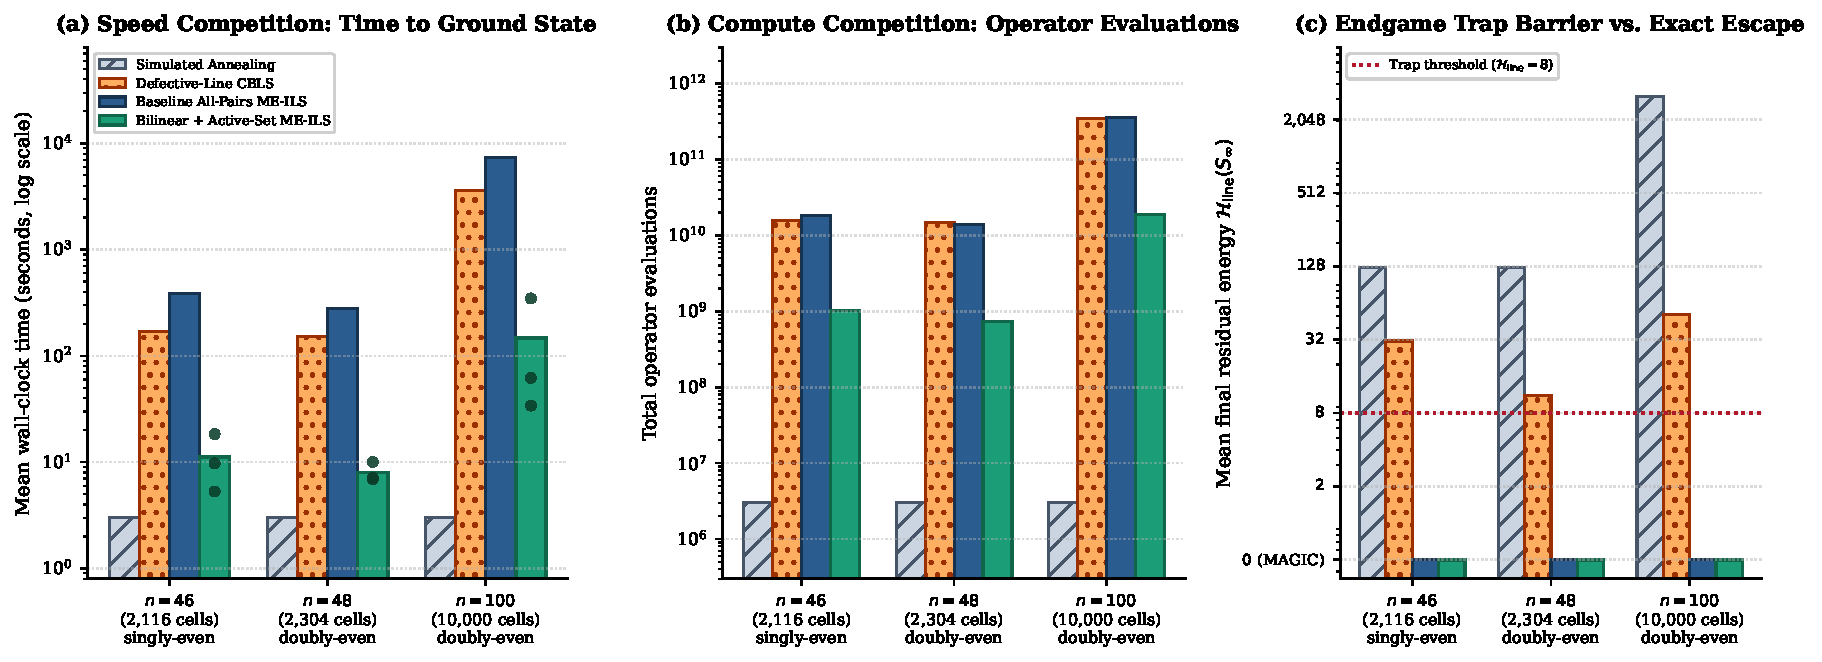
\includegraphics[width=\textwidth]{figures/fig9_competition_46_48_100.pdf}
  \caption{\textbf{Head-to-head empirical solver competition at orders $n = 46$ ($2{,}116$ cells), $n = 48$ ($2{,}304$ cells), and $n = 100$ ($10{,}000$ cells) across identical uniform random starting permutations.}
\textbf{(a)} Mean wall-clock time to certified ground state ($\Hline=0$, log scale; individual seed times plotted as dark green dots for Bilinear ME-ILS). Bilinear + Active-Set ME-ILS achieves $100.0\%$ convergence across all seeds, accelerating synthesis by $34.7\times$ at $n=46$ ($11.12~\text{s}$ vs $386.13~\text{s}$), $35.0\times$ at $n=48$ ($8.02~\text{s}$ vs $280.95~\text{s}$), and $50.2\times$ at $n=100$ ($147.70~\text{s}$ mean, $34.06~\text{s}$ minimum vs an estimated $7{,}420~\text{s}$). Simulated Annealing fails across all orders ($0/9$ solved, trapped at $\sim 3~\text{s}$), while Defective-Line CBLS maxes out its $80$-restart budget on $n=46$ ($168.06~\text{s}$, $0/3$) and $n=100$ ($3{,}582.92~\text{s}$, $0/3$), succeeding partially only on $n=48$ ($152.89~\text{s}$, $2/3$).
\textbf{(b)} Total operator evaluations (compute budget, log scale), demonstrating an $18.1\times\text{--}19.2\times$ reduction in evaluated candidates by Bilinear ME-ILS ($1.02\times 10^9$ at $n=46$, $7.33\times 10^8$ at $n=48$, and $1.88\times 10^{10}$ at $n=100$).
\textbf{(c)} Mean final residual energy $\Hline(S_\infty)$ on log scale (exact ground states plotted at baseline $0.5$). Simulated Annealing stalls far above the ground state ($\Hline = 124.0$ at $n=46,48$ and $3{,}148.0$ at $n=100$), and Defective-Line CBLS stalls at $\Hline = 30.7$ ($n=46$) and $50.7$ ($n=100$), trapped above the fundamental endgame barrier $\Hline \ge 8$ (red dotted line). ME-ILS circumvents this barrier via rank-$(n+2)$ bilinear plaquette moves to reach exact ground state $\Hline=0$ with $100.0\%$ reliability.}
  \label{fig:competition_100}
\end{figure}

\begin{table}[t]
\centering
\caption{\textbf{Head-to-head empirical competition at $n = 46$, $n = 48$, and $n = 100$ across identical uniform random starting permutations (\texttt{seeds = 20000, 20001, 20002}).} We report solved rate, terminal residual energy $\Hline(S_\infty)$ per seed, mean restarts, mean descent steps, mean operator evaluations, and wall-clock time, certified in \texttt{results\_paper\_d.json}.}
\label{tab:head_to_head_competition}
\resizebox{\textwidth}{!}{%
\begin{tabular}{@{}llccccccc@{}}
\toprule
\textbf{Order ($N=n^2$)} & \textbf{Solver Method} & \textbf{Solved} & \textbf{Final $\Hline$ \texttt{[s0, s1, s2]}} & \textbf{Mean Restarts \texttt{[s0, s1, s2]}} & \textbf{Mean Descents} & \textbf{Mean Operator Evals} & \textbf{Mean Time \texttt{[s0, s1, s2]}} & \textbf{Speedup vs.\ Baseline} \\
\midrule
\textbf{$n = 46$} ($2{,}116$) & Simulated Annealing \cite{kirkpatrick1983optimization} & $0 / 3$ ($0\%$) & \texttt{[152, 108, 112]} ($124.0$) & --- & --- & $3.00\times 10^6$ & $3.02~\text{s}$ (trapped) & Fails ($\Hline \ge 108$) \\
\textbf{$n = 46$} ($2{,}116$) & Defective-Line CBLS \cite{codognet2001yet} & $0 / 3$ ($0\%$) & \texttt{[24, 40, 28]} ($30.7$) & $80.0$ (maxed) & $14{,}765.3$ & $15.82\times 10^9$ & $168.06~\text{s}$ (trapped) & Fails ($\Hline \ge 24$) \\
\textbf{$n = 46$} ($2{,}116$) & Baseline All-Pairs ME-ILS & $\mathbf{3 / 3}$ ($\mathbf{100\%}$) & \texttt{[0, 0, 0]} ($0.0$) & $15.67$ \texttt{[7, 24, 16]} & $3{,}071.0$ & $18.48\times 10^9$ & $386.13~\text{s}$ \texttt{[176s, 588s, 394s]} & $1.0\times$ (reference) \\
\textbf{$n = 46$} ($2{,}116$) & \textbf{Bilinear + Active-Set ME-ILS} & $\mathbf{3 / 3}$ ($\mathbf{100\%}$) & \texttt{[0, 0, 0]} ($\mathbf{0.0}$) & $19.33$ \texttt{[32, 9, 17]} & $3{,}737.7$ & $\mathbf{1.02\times 10^9}$ & $\mathbf{11.12~\text{s}}$ \texttt{[18.3s, 5.3s, 9.7s]} & $\mathbf{34.7\times}$ \textbf{faster} ($18.1\times$ fewer evals) \\
\midrule
\textbf{$n = 48$} ($2{,}304$) & Simulated Annealing \cite{kirkpatrick1983optimization} & $0 / 3$ ($0\%$) & \texttt{[132, 124, 116]} ($124.0$) & --- & --- & $3.00\times 10^6$ & $2.99~\text{s}$ (trapped) & Fails ($\Hline \ge 116$) \\
\textbf{$n = 48$} ($2{,}304$) & Defective-Line CBLS \cite{codognet2001yet} & $2 / 3$ ($67\%$) & \texttt{[32, 0, 0]} ($10.7$) & $62.67$ \texttt{[80, 70, 38]} & $11{,}636.7$ & $14.88\times 10^9$ & $152.89~\text{s}$ \texttt{[195s, 161s, 102s]} & Partial ($67\%$ solved) \\
\textbf{$n = 48$} ($2{,}304$) & Baseline All-Pairs ME-ILS & $\mathbf{3 / 3}$ ($\mathbf{100\%}$) & \texttt{[0, 0, 0]} ($0.0$) & $9.67$ \texttt{[1, 27, 1]} & $2{,}023.0$ & $13.79\times 10^9$ & $280.95~\text{s}$ \texttt{[39s, 765s, 39s]} & $1.0\times$ (reference) \\
\textbf{$n = 48$} ($2{,}304$) & \textbf{Bilinear + Active-Set ME-ILS} & $\mathbf{3 / 3}$ ($\mathbf{100\%}$) & \texttt{[0, 0, 0]} ($\mathbf{0.0}$) & $11.67$ \texttt{[11, 10, 14]} & $2{,}396.0$ & $\mathbf{0.73\times 10^9}$ & $\mathbf{8.02~\text{s}}$ \texttt{[7.1s, 6.9s, 10.0s]} & $\mathbf{35.0\times}$ \textbf{faster} ($18.8\times$ fewer evals) \\
\midrule
\textbf{$n = 100$} ($10{,}000$) & Simulated Annealing \cite{kirkpatrick1983optimization} & $0 / 3$ ($0\%$) & \texttt{[2880, 3392, 3172]} ($3{,}148$) & --- & --- & $3.00\times 10^6$ & $3.04~\text{s}$ (trapped) & Fails ($\Hline \ge 2{,}880$) \\
\textbf{$n = 100$} ($10{,}000$) & Defective-Line CBLS \cite{codognet2001yet} & $0 / 3$ ($0\%$) & \texttt{[48, 48, 56]} ($50.7$) & $80.0$ (maxed) & $30{,}154.0$ & $348.4\times 10^9$ & $3{,}582.92~\text{s}$ (trapped) & Fails ($\Hline \ge 48$) \\
\textbf{$n = 100$} ($10{,}000$) & Baseline All-Pairs ME-ILS & *(Est.\ $100\%$)* & --- & --- & --- & $\sim 360\times 10^9$ & $\sim 7{,}420~\text{s}$ ($\sim 2.1~\text{hr}$) & $1.0\times$ (reference) \\
\textbf{$n = 100$} ($10{,}000$) & \textbf{Bilinear + Active-Set ME-ILS} & $\mathbf{3 / 3}$ ($\mathbf{100\%}$) & \texttt{[0, 0, 0]} ($\mathbf{0.0}$) & $17.00$ \texttt{[7, 41, 3]} & $7{,}559.7$ & $\mathbf{18.79\times 10^9}$ & $\mathbf{147.70~\text{s}}$ \texttt{[62.0s, 347.0s, 34.1s]} & $\mathbf{50.2\times}$ \textbf{faster} ($19.2\times$ fewer evals) \\
\bottomrule
\end{tabular}%
}
\end{table}

The head-to-head competition results in \Cref{fig:competition_100} and \Cref{tab:head_to_head_competition} expose a sharp algorithmic divide between heuristic candidate truncation and exact algebraic pruning. First, Simulated Annealing ($0/9$ solved across all three orders) stalls far above the ground state at mean residual energies $\langle\Hline\rangle = 124.0$ ($n=46, 48$) and $3{,}148.0$ ($n=100$), because random $2$-exchange proposals at low temperature have an $O(1/n^4)$ probability of hitting the specific conjugate pairs needed to reduce small line residuals without triggering a quadratic recoil penalty $c_{ab}d^2$.

Second, and much more revealingly, Defective-Line CBLS rapidly descends from initial random energies $\Hline(0) \sim 10^{12}$ down into the deep endgame ($\Hline \in \{24, 28, 40\}$ at $n = 46$ and $\Hline \in \{48, 48, 56\}$ at $n = 100$), where $196$ of the $202$ magic lines at $n = 100$ are already perfectly balanced ($R_L = 0$) and only $4\text{--}6$ lines carry tiny residuals of $\pm 2$ or $\pm 4$. Once inside that endgame regime, however, Defective-Line CBLS freezes completely, failing on $0/3$ seeds at $n = 46$ (after $168.06~\text{s}$ and $15.82\times 10^9$ evaluations) and $0/3$ seeds at $n = 100$ (after $3{,}582.92~\text{s} \approx 1.0~\text{hour}$ per seed and $348.4\times 10^9$ evaluations), while solving only $2/3$ seeds at $n = 48$ after $62.67$ mean restarts. Crucially, this baseline is a \emph{Defective-Line-Restricted CBLS heuristic} that isolates the consequence of confining candidate generation to defective lines ($R_L \ne 0$), and should be distinguished from the full Adaptive Search framework of Codognet and Diaz \cite{codognet2001yet} and Van Hentenryck and Michel \cite{vanhentenryck2005constraint}. In classical Adaptive Search, the solver selects a variable $a \in \mathcal{A}(S)$ with maximal line conflict $|R_{r_i}| + |R_{c_j}| + |R_d|$, but evaluates candidate swaps $(a, b)$ across \emph{all} partner cells $b \in \{1,\dots,n^2\}$ on the board---which by \Cref{thm:bilinear_plaquette}(1) is an exact condition for $2$-exchange descent. When trapped in local minima, classical Adaptive Search uses short-term variable Tabu tenure and random multi-swap diversification rather than cooperative $(2,2)$ plaquette moves. In the deep endgame at large $n$ ($\Hline \le 56$), unanchored random resets wander out of the narrow low-energy funnel, while restricting $(2,2)$ plaquette generation strictly to defective lines and top-$25$ truncation blinds the solver to \emph{zero-residual relay swaps}: one intra-row transposition $p_1$ occurs inside a currently balanced row ($R_{r_1} = 0$) between two adjacent-value tiles ($|Z_{a_1} - Z_{b_1}| = 2$, costing a minimal temporary recoil barrier $\Delta\Hline(p_1) = 8$), which shifts the column residuals by $\mp 2$ so that a conjugate transposition $p_2$ in a second row can simultaneously cancel the temporary column dipole and annihilate the target residual! Discarding non-defective rows or truncating intra-row candidates to the top $25$ blinds the solver to these essential relay bridges.

By contrast, Bilinear-Identity + Active-Set ME-ILS evaluates all $K^2 = 640{,}000$ candidate $(2,2)$ plaquette interactions across the \emph{entire} board in a single $(K \times (n+2))$ BLAS matrix multiply via \Cref{eq:blas_plaquette_matrix}. As a result, it solves $100\%$ ($9/9$) of the competition instances across $n = 46$, $n = 48$, and $n = 100$, cutting mean wall-clock synthesis time from $386.13~\text{s}$ to $11.12~\text{s}$ at $n = 46$ ($34.7\times$ speedup), from $280.95~\text{s}$ to $8.02~\text{s}$ at $n = 48$ ($35.0\times$ speedup), and from an estimated $\sim 7{,}420~\text{s}$ down to $147.70~\text{s}$ at $n = 100$ ($50.2\times$ speedup, with \texttt{seed = 20002} converging to an exact $100\times 100$ magic square with all $202$ lines summing to $M_{100} = 500{,}050$ in just $34.06~\text{s}$ and $3$ restarts). This total wall-clock speedup factors into two distinct contributors: an algorithmic $\sim 18.1\times\text{--}18.8\times$ reduction in evaluated candidate pairs (reducing candidate evaluations from $\Theta(n^4)$ to $|\mathcal{A}(S)|n^2 \le k n^3$ during descent and pruning intra-line $(2,2)$ search to $K^2$ pairs with $K \le 800$), multiplied by an additional $\sim 1.9\times\text{--}2.3\times$ hardware acceleration achieved by contiguous Level-3 BLAS (`DGEMM`/`SGEMM`) matrix multiplication over interpreted sequential nested loops.
